\documentclass[9pt, technote]{IEEEtran}
\usepackage[table]{xcolor}
\usepackage[numbers]{natbib}
\usepackage{graphicx}
\usepackage{listings}
\usepackage{caption}
\usepackage{subcaption}
\usepackage{pgf}
\usepackage[most]{tcolorbox}
%\usepackage[margin=1in]{geometry}
\usepackage{inconsolata}
\usepackage{cleveref}
\let\labelindent\relax
\usepackage[inline]{enumitem}
\usepackage{dcolumn}
\usepackage{booktabs}
\usepackage{subfig}

%\usepackage[scaled]{helvet}
%\renewcommand\familydefault{\sfdefault} 
%\usepackage[T1]{fontenc}

\definecolor{lightgray}{rgb}{.9,.9,.9}
\definecolor{darkgray}{rgb}{.4,.4,.4}
\definecolor{purple}{rgb}{0.65, 0.12, 0.82}
\definecolor{atomred}{RGB}{224, 108, 117}
\definecolor{atomwhite}{RGB}{250, 250, 250}


\lstdefinelanguage{JavaScript}{
  keywords={typeof, new, true, false, catch, function, return, null, catch, switch, var, if, in, while, do, else, case, break},
  keywordstyle=\color{blue}\bfseries,
  ndkeywords={class, export, boolean, throw, implements, import, this},
  ndkeywordstyle=\color{darkgray}\bfseries,
  identifierstyle=\color{black},
  sensitive=false,
  comment=[l]{//},
  morecomment=[s]{/*}{*/},
  commentstyle=\color{purple}\ttfamily,
  stringstyle=\color{atomred}\ttfamily,
  morestring=[b]',
  morestring=[b]"
}

\lstset{
   language=JavaScript,
   backgroundcolor=\color{white},
   extendedchars=true,
   basicstyle=\ttfamily\footnotesize,
   showstringspaces=false,
   showspaces=false,
   numbers=left,
   numberstyle=\ttfamily\footnotesize,
   numbersep=5pt,
   tabsize=2,
   breaklines=true,
   showtabs=false,
   captionpos=b,
   frame=single
}

\begin{document}

\title{On the Performance of String Search Algorithms for Deep Packet Inspection}
\date{\today}
\maketitle

\abstract{As the speed of computer processors grows, so too does the speed at which networks communicate \citep{neilsen1998}. With more and more people placing increasing trust on computer networks, the requirement for safety within these networks is paramount. Traditionally, packet analysis in firewalls and intrusion detection systems has been achieved through expensive and custom hardware specifically designed for this purpose. Off-the-shelf hardware - although slower - makes it easier for implementers to quickly develop and deploy new packet inspection techniques and rules, and create systems that scale to meet a network's demands. This paper investigates and compares exact string matching algorithms - implemented on general purpose processors - for the purpose of deep packet inspection.}

\section{Introduction}

Deep Packet Inspection (DPI) systems today are designed to operate on expensive custom hardware \citep{abuhmed2007}. Making changes to such a system (such as horizontally or vertically scaling) is often arduous, time consuming and expensive; the process requires adding or removing hardware that is often made-to-order from a manufacturer. Deep Packet Inspection via software means is slower but does provide some benefit over that of hardware inspection. Increasing the speed of software-based Deep Packet Inspection is often as simple as increasing the number of hosts performing the inspection \citep{chaudhary2011}. Modern data centres using hardware virtualisation enable the provisioning of extra processing capacity to done with very little lead time and to be completed quickly. This allows resources to only be used when needed and used elsewhere when not. 

String search algorithms have long been of interest to the field of computer science - with the first paper being 1970 \citep{morris1970} - and as a result a substantial number of search algorithms exist \cite{charras2004}. The following paper asks which of these string search algorithms performs best at Deep Packet Inspection and how does their performance compare to that of their theoretical speed.

In order to properly test these string search algorithms, a system was designed to accurately compare each algorithm for inspection of both packet captures as well as textual inputs such as text files.

\section{Background}

In the context of Deep Packet Inspection, the following definitions are relevant:
\begin{itemize}
  \item \underline{Packet}: Binary data representing a unit of data carried on a packet-switched network . This includes information from the network to the application layer. The word \textit{packet} is overloaded in computer networking: it either refers to the data unit containing Network Layer information in the OSI model, the data unit containing Network layer information in the TCP/IP model or an entire unit of data transmitted over a network. When referring to a packet we imply the latter meaning.
  \item \underline{Packet Capture File (PCAP)}: A file containing packets. These packets were generally captured by recording a network interface using the libpcap library \citep{tcpdump2016}.
  \item \underline{Deep Packet Inspection (DPI)}: The process by which a PCAP file or stream of packets from a network interface, is analysed for the presence of predefined patterns or rules.
\end{itemize}

\subsection{String Search Algorithms}

A vast collection of string search algorithms have been described by Charras and Lecroq \citep{charras2004}, and from that a selection of algorithms was chosen to implement, benchmark and then compare. These algorithms share a number similarities:
\begin{itemize}
  \item \underline{Exact String Matching}: Each of the algorithms that have been chosen to compare exactly match a given rule or pattern in an input. Some string search algorithms are designed to show partial matches but none of these have been selected for comparison.
  \item \underline{Single Rule Matching}: Each of these algorithms searches for just a single rule throughout the entire input. For multiple rules another solution is needed.
\end{itemize}

Rules take the form of a string which is then search for in the input.

Table \ref{table-algorithms} has a list of each algorithm, the year it was publish, its author(s) and the time complexity of searching with that algorithm.

\begin{table}[!hbt]
\centering
\caption{Implemented string search algorithms for the purpose of comparison against a packet dataset. Under time complexity, \textit{n} represents the length of the Input and \textit{m} represents the length of a Rule. The time complexity is multiplied by a factor equal to the number of Rules.}
\label{table-algorithms}
\resizebox{\ifdim\width>\columnwidth\columnwidth\else\width\fi}{!}{
\begin{tabular}{@{}llll@{}}
\toprule
Algorithm & Year & Cite & Big-0 \\ \midrule
Naive &  &  & O(mn) \\
MorrisPratt & 1970 & \citep{morris1970} & $O(n + m)$ \\
KnuthMorrisPratt & 1977 & \citep{knuth1977} & $O(n + m)$ \\
BoyerMoore & 1977 & \citep{boyer1977} & $O(nm)$ \\
Horspool & 1980 & \citep{horspool1980} & $O(n + m)$ \\
ApostolicoGiancarlo & 1986 & \citep{apostolico1986} & $O(n)$ \\
RabinKarp & 1987 & \citep{karp1987} & $O(nm)$ \\
ZhuTakaoka & 1987 & \citep{feng1987} & $O(nm)$ \\
QuickSearch & 1990 & \citep{sunday1990} & $O(nm)$ \\
Smith & 1991 & \citep{smith1991} & $O(nm)$ \\
ApostolicoCrochemore & 1991 & \citep{apostolico1991} & $O(n)$ \\
Colussi & 1991 & \citep{colussi1991} & $O(n)$ \\
Raita & 1991 & \citep{raita1991} & $O(nm)$ \\
GalilGiancarlo & 1991 & \citep{galil1991} & $O(n)$ \\
Bitap (Shift Or) & 1992 & \citep{baezayates1992} & $O(n)$ \\
NotSoNaive & 1993 & \citep{hancart1993} & $O(nm)$ \\
Simon & 1994 & \citep{simon1994} & $O(n + m)$ \\
TurboBoyerMoore & 1994 & \citep{crochemore1994} & $O(n)$ \\
ReverseColussi & 1994 & \citep{colussi1994} & $O(n)$ \\ \bottomrule
\end{tabular}}
\end{table}

Each of the string search algorithms has a known theoretical performance, known as algorithm complexity or  `Big-O'. The algorithmic complexity is used to describe the behaviour of an algorithm as its factors tend towards infinity \citep{bachman1894, landau1909}. This value is generally related in some way to both the length of the input and rule. The results of the following experiments should follow the predicted complexity of string search algorithms. Algorithm complexity often only provides insight into processing speed where large variations in Input length (differing orders of magnitude) are present. In packet data a limited range of input lengths is possible - this value is set by the maximum transmission unit of the transport medium - and so it may come down to minutiae within the algorithms themselves rather than their overall complexity.

As the implemented algorithms were designed to search for a single rule, their Big-O notations only reflect that property. For many rules, and a serial-style programming approach (each rule is searched for sequentially), these algorithms need to run back-to-back; this style of implementation increases their time to process by a factor about equal to the number of rules. For a parallel-style approach (where many rules are searched for at the same time) the processing time is affected by a factor lower than that of the serial implementation. The speed at which a search for a complete set of rules with a parallel implementation completes is then both related to the algorithmic complexity of the search as well as the number of rules which are being searched for at the same time.

An upper bound for the number of concurrent searches for different rules with the same algorithm and input does exist. That upper bound is defined by the number of processor cores that are available for use as how much a single thread is able to saturate a processor core.
For a system with 10 cores. Running a search in a single thread (and therefor on a single core) is only using 10\% of the available processing power. Splitting the search across 10 should serve to give close to an order of magnitude speed increase. If those threads were saturating the processing speed of all 10 cores (using 100\% of the available processing power), adding more threads might serve to reduce the benefits seen before. The overhead of switching between threads on a single core may start to adversely affect the processing time.

\section{Method}

For the purpose of these experiments, a system was developed to allow for the accurate running and performance measurement of each of the implemented algorithms (in Table \ref{table-algorithms}). 
The following terminology is relevant to that system:
\begin{itemize}
  \item \textbf{Input}: The system interacts with all kinds of input through a common interface. Both textual- and packet-style are interacted with through this interface. The system is able to request a single byte of data at a given location from an input as well as obtain the length of the input.
  \item \textbf{Rule}: Rules are the patterns searched for by the system. Rules mimic inputs in that the system may also retrieve a single byte from the rule or get the rule's length.
  \item \textbf{Algorithm}: This represents a string search algorithm (from Table \ref{table-algorithms}) and is the means by which the system interacts with all of the implemented algorithms. An algorithm provides a search function to the system with common inputs and outputs.
  \item \textbf{Result}: For a single input, set of rules and a particular run, a result is created. This result contains all of the information about the outcome of the search and the configuration surrounding it.
\end{itemize}

The test system was designed to accept a JSON file \citep{json2016} as configuration (shown in Listing \ref{listing-testConfiguration.json}).
\begin{lstlisting}[caption=Sample testConfiguration.json, label=listing-testConfiguration.json, linewidth=\columnwidth, xleftmargin=5.0ex]
{
  "algorithms": ["Naive", "MorrisPratt", ..., "ReverseColussi"],
  "rules": ["time", "person", ..., "msn"],
  "inputs": [
    {
      "type": "pcap",
      "location": "smallcapture.pcap"
    },
    {
      "type": "text",
      "location": "alice.txt"
    }
  ],
  "times": 20,
  "threadCount": 18
}
\end{lstlisting}

For the test, the following configuration was chosen:
\begin{itemize}
  \item \texttt{algorithms} - a list of all implemented algorithms (See Table \ref{table-algorithms}) 
  \item \texttt{rules} - string-based rules covering the twenty most popular websites \citep{alexa2016} - where just their domain names were taken - as well as the twenty most popular words in the English language \citep{oed2016}.
  \item \texttt{inputs} - a dataset of DNS traffic was selected and a subset of 10000 packets was extracted. This was labeled \texttt{smallcapture.pcap} and known hereafter as \textit{Dataset A}. The complete \textit{Alice in Wonderland} by Lewis Carol, labeled as labeled \texttt{alice.txt}, was selected as the second input and known hereafter as \textit{Dataset B}. The test system treats textual and PCAP input files differently. Text input files transformed into a single input object representing all information in that file. PCAP input files are split up into individual packet objects and each packet represents a single input.
  \item \texttt{times} - each algorithm searched all inputs for every rule. We chose to repeat the test 20 times to ensure that transient fluctuations caused by other processes on the test hardware could be identified.
  \item \texttt{threadCount} - drastic speed increases are made possible by splitting the work of the Algorithms across multiple threads. The machine used to perform the test has 24 useable cores and so a max \texttt{threadCount} of 18 was chosen to best make use of those cores. 
\end{itemize}


For \textit{Dataset A}, \ref{table-inputsummary} gives a statistical summary of the lengths of the inputs. As \textit{Dataset A} is comprised of DNS requests and responses it is unsurprising that the average length of a packet is about 110 bytes. This is far below the ethernet maximum transmission unit of 1500 bytes \citep{rfc894}. 

\begin{table}[!htb]
  \centering
  \resizebox{\ifdim\width>\columnwidth\columnwidth\else\width\fi}{!}{
  \begin{tabular}{cccccc}
    Minimum & First Quartile & Median & Mean & Third Quartile & Maximum \\
    \hline
    54.0 & 81.0 & 85.0 & 109.8 & 99.0 & 585.0
  \end{tabular}}
  \caption{\textit{Dataset A} packet length statistical summary (in bytes).}
  \label{table-inputsummary}
\end{table}


\section{Results}

The test generated 340 0340 result objects. Result objects look similar to Listing \ref{listing-testresult}. Each result object contains the following information about a search: the start time and end time, the elapsed time ($ end\ time - start\ time $), the list of rules, the locations that the rules were found in the input, the algorithm used to perform the search, the input file (as mentioned earlier many inputs can share an input file), the unique ID of the input, the run number (between 1 and the number of times the test was set to run), and the ID of that run.

\begin{lstlisting}[caption=Example result, label=listing-testresult, linewidth=\columnwidth, xleftmargin=5.0ex]
[
    {
        "start": 206079193307938,
        "end": 206079207132342,
        "elapsed": 13824404,
        "rules": ["time", "person", ... "msn"],
        "locations": [1, 2, ..., n],
        "algorithm": "Smith",
        "inputFile": "smallcapture.pcap",
        "inputID": "bf75faa5",
        "runNumber": 1,
        "runId": "d9b4a28aefbd"
    },
    ...
]
\end{lstlisting}

\subsection{Analysis}

In order to accurately judge the performance of the string search algorithms in the context of Deep Packet Inspection, a number of questions relating to their behaviour were posed. First and foremostly is the question of the algorithms' raw speed when processing the datasets. Next, an indication of the algorithms' behaviour for inputs of varying length was needed. Algorithms should be able to process each packet - regardless of length - in a reasonable amount of time. Finally, algorithms must have deterministic processing times for good candidacy in packet processing. An indication of determinism is the standard deviation of each algorithm. 

\subsubsection{Which Algorithms are Fastest? Which are Slowest?}

Figure \ref{figure-barmeanprocessingsmallcapture} shows a comparison of processing times for each algorithm over each of the packets in \textit{Dataset A}. Figure \ref{figure-barmeanprocessingalice} gives the same comparison, this time where \textit{Dataset B} is the input.

\begin{figure}[!htb]
    \centering
    \begin{subfigure}[b]{\columnwidth}
        \centering
        \includegraphics[width=\textwidth]{images/bar_graph_mean_one_input_smallcapture_pcap}
        \caption{Mean Input processing times of each Algorithm for \textit{PCAP Dataset}.}
        \label{figure-barmeanprocessingsmallcapture}
    \end{subfigure}
    ~
    \begin{subfigure}[b]{\columnwidth}
        \centering
        \includegraphics[width=\textwidth]{images/bar_graph_mean_one_input_alice_txt} 
        \caption{Mean Input processing times of each Algorithm for \textit{Alice in Wonderland}.}
        \label{figure-barmeanprocessingalice}
    \end{subfigure}
    \caption{Mean input processing times for each algorithm.}
\end{figure}

The order of the algorithms in Figures \ref{figure-barmeanprocessingsmallcapture} and \ref{figure-barmeanprocessingalice} is inconsistent. The relative position of each algorithm, from one figure to the other varies by very little. The relative speed difference of each algorithm in Figure \ref{figure-barmeanprocessingsmallcapture} is noticeably small in comparison with the slowest algorithm. The first sixteen algorithms appear to have nearly identical mean processing speeds. By increasing the length of the input data (in this case by using the \textit{Dataset B} in Figure \ref{figure-barmeanprocessingalice}) we are able to accentuate the differences between the algorithms.

Table \ref{table-algorithmspeed} gives a full statistical summary of every algorithm searching through \textit{Dataset A}.\\

\begin{table}[!hbt]
\centering
\caption{Algorithm processing time statistics for \textit{Dataset A}}
\label{table-algorithmspeed}
\resizebox{\columnwidth}{!}{%
\begin{tabular}{@{}rllllll@{}}
\toprule
Algorithm & \multicolumn{1}{c}{Min} & \multicolumn{1}{c}{Q\textsubscript{1}} & \multicolumn{1}{c}{$\widetilde{\Delta{t}}$} & \multicolumn{1}{c}{$\mu$} & \multicolumn{1}{c}{Q\textsubscript{3}} & \multicolumn{1}{c}{Max} \\ \midrule
\rowcolor[HTML]{67FD9A} 
\multicolumn{1}{r|}{\cellcolor[HTML]{67FD9A}QuickSearch} & 0.08321 & 0.10750 & 0.11430 & 0.16350 & 0.12320 & \multicolumn{1}{r}{259.7} \\
\rowcolor[HTML]{67FD9A} 
\multicolumn{1}{r|}{\cellcolor[HTML]{67FD9A}Horspool} & 0.0926 & 0.1098 & 0.1166 & 0.1640 & 0.1246 & \multicolumn{1}{r}{5.337} \\
\multicolumn{1}{r|}{ReverseColussi} & 0.09139 & 0.11180 & 0.11910 & 0.16410 & 0.12740 & 5.7 \\
\multicolumn{1}{r|}{Raita} & 0.09035 & 0.10710 & 0.11600 & 0.16560 & 0.12440 & 164.1 \\
\multicolumn{1}{r|}{ZhuTakaoka} & 0.09288 & 0.11200 & 0.11900 & 0.16560 & 0.12740 & 4.645 \\
\multicolumn{1}{r|}{KnuthMorrisPratt} & 0.09113 & 0.11180 & 0.11930 & 0.16630 & 0.12780 & 25.96 \\
\multicolumn{1}{r|}{Colussi} & 0.09178 & 0.11130 & 0.11840 & 0.16640 & 0.12670 & 29.69 \\
\multicolumn{1}{r|}{Smith} & 0.09102 & 0.11170 & 0.11880 & 0.16710 & 0.12660 & 5.334 \\
\multicolumn{1}{r|}{BoyerMoore} & 0.09287 & 0.11070 & 0.11740 & 0.16730 & 0.12540 & 33.22 \\
\multicolumn{1}{r|}{MorrisPratt} & 0.08543 & 0.10910 & 0.11540 & 0.16750 & 0.12360 & 297.8 \\
\multicolumn{1}{r|}{Naive} & 0.08845 & 0.11180 & 0.11830 & 0.16820 & 0.12620 & 63.84 \\
\multicolumn{1}{r|}{Bitap} & 0.09277 & 0.11160 & 0.11900 & 0.16840 & 0.12780 & 50.14 \\
\multicolumn{1}{r|}{TurboBoyerMoore} & 0.09101 & 0.11220 & 0.11900 & 0.16880 & 0.12680 & 41.68 \\
\rowcolor[HTML]{96FFFB} 
\multicolumn{1}{r|}{\cellcolor[HTML]{96FFFB}RabinKarp} & 0.09562 & 0.11580 & 0.12230 & 0.17070 & 0.13200 & \multicolumn{1}{r}{245.6} \\
\multicolumn{1}{r|}{Simon} & 0.08248 & 0.11140 & 0.11890 & 0.17320 & 0.12750 & 117.2 \\
\multicolumn{1}{r|}{ApostolicoGiancarlo} & 0.09368 & 0.11420 & 0.12170 & 0.17340 & 0.13020 & 5.067 \\
\rowcolor[HTML]{96FFFB} 
\multicolumn{1}{r|}{NotSoNaive} & 0.1092 & 0.1698 & 0.2277 & 0.3806 & 0.2957 & \multicolumn{1}{r}{552.3} \\ \bottomrule
\end{tabular}%
}
\end{table}

In Table \ref{table-algorithmspeed}, the the fastest algorithms from Figures \ref{figure-barmeanprocessingsmallcapture} and \ref{figure-barmeanprocessingalice} are highlighted in green whilst the two slowest algorithms from those figures are highlighted in blue.

The slowest algorithms from those tests were the Not So Na\"ive \citep{hancart1993} and Rabin-Karp \cite{karp1987} algorithms. The fastest algorithms were the Quick Search \citep{sunday1990} and Horspool \citep{horspool1980} algorithms.

The QuickSearch \citep{sunday1990} algorithm makes use of the BoyerMoore \citep{boyer1977} algorithm's bad-character shift table \citep{charras2004}. The algorithm is known to perform well for short rules \citep{leqroc1995}. Our test consisted primarily of fairly short rules which may indicate why the algorithm performed so well.

The Horspool \citep{horspool1980} algorithm also makes use of the bad-character shift table from the BoyerMoore \citep{boyer1977} algorithm. Although the Horspool algorithm has a $O(nm)$ complexity (Table \ref{table-algorithms}), it can be shown that the average number of comparisons made with a character in the input is $\alpha$, where $\frac{1}{c} \leq \alpha \leq \frac{2}{c+1}$ and $c$ is the number of characters in the alphabet \citep{baezayates1992b}. In our case our alphabet is 256 characters long (the size of one byte) making the average number of comparisons to a character in our text $0.0039 \leq \alpha \leq 0.0079$. That is a very low number of comparisons per input character.\\

RabinKarp's \citep{karp1987} slowness can easily be attributed to both its O(mn) complexity as well as its constant recalculation of the input hash. The RabinKarp algorithm works by maintaining a hash of the rule and calculating a hash on a sliding window of the input. The theory is that the comparison between the hashes is faster than that of the entire rule with the sliding window each time.

NotSoNaive's \citep{hancart1993} slowness is surprising at first. It performs worse than the Naive algorithm when it was designed as an improvement on it. The NotSoNaive algorithm attempts to improve upon the Naive algorithm by adding a check to see if the input ahead shows signs of matching the rule; this extra step seems to cause the speed decrease when compared to Naive. Figure \ref{table-algorithmspeed} may make you may think that the mean processing time for NotSoNaive was heavily influenced by the maximum speed (that is to say that that maximum value is an outlier. Table \ref{table-algorithmspeed}) but by checking the median processing time - again in \ref{table-algorithmspeed} - it is clear that the entire set of results is shifted towards a longer processing time.

\subsubsection{Do Some Algorithms Perform Differently Depending on the Input Length?}

Figure \ref{figure-speedvslength} shows a scatter plot of mean input processing time versus packet length. This plot shows processing times for all algorithms. Note that the vertical axis has been plotted with a logarithmic scale. From the plot it is clear that there is an upward trend of processing time as the input length increases. This is expected as every algorithm in Table \ref{table-algorithms} has an algorithmic complexity related to the length of the input.

\begin{figure}[!htb]
    \centering
    \includegraphics[width=\columnwidth]{images/scatter_mean_time_vs_input_length_pcap}
    \caption{Input processing speeds vs input length for \textit{Dataset A}.}
    \label{figure-speedvslength}
\end{figure}

\begin{figure}[!hbt]
  \centering
  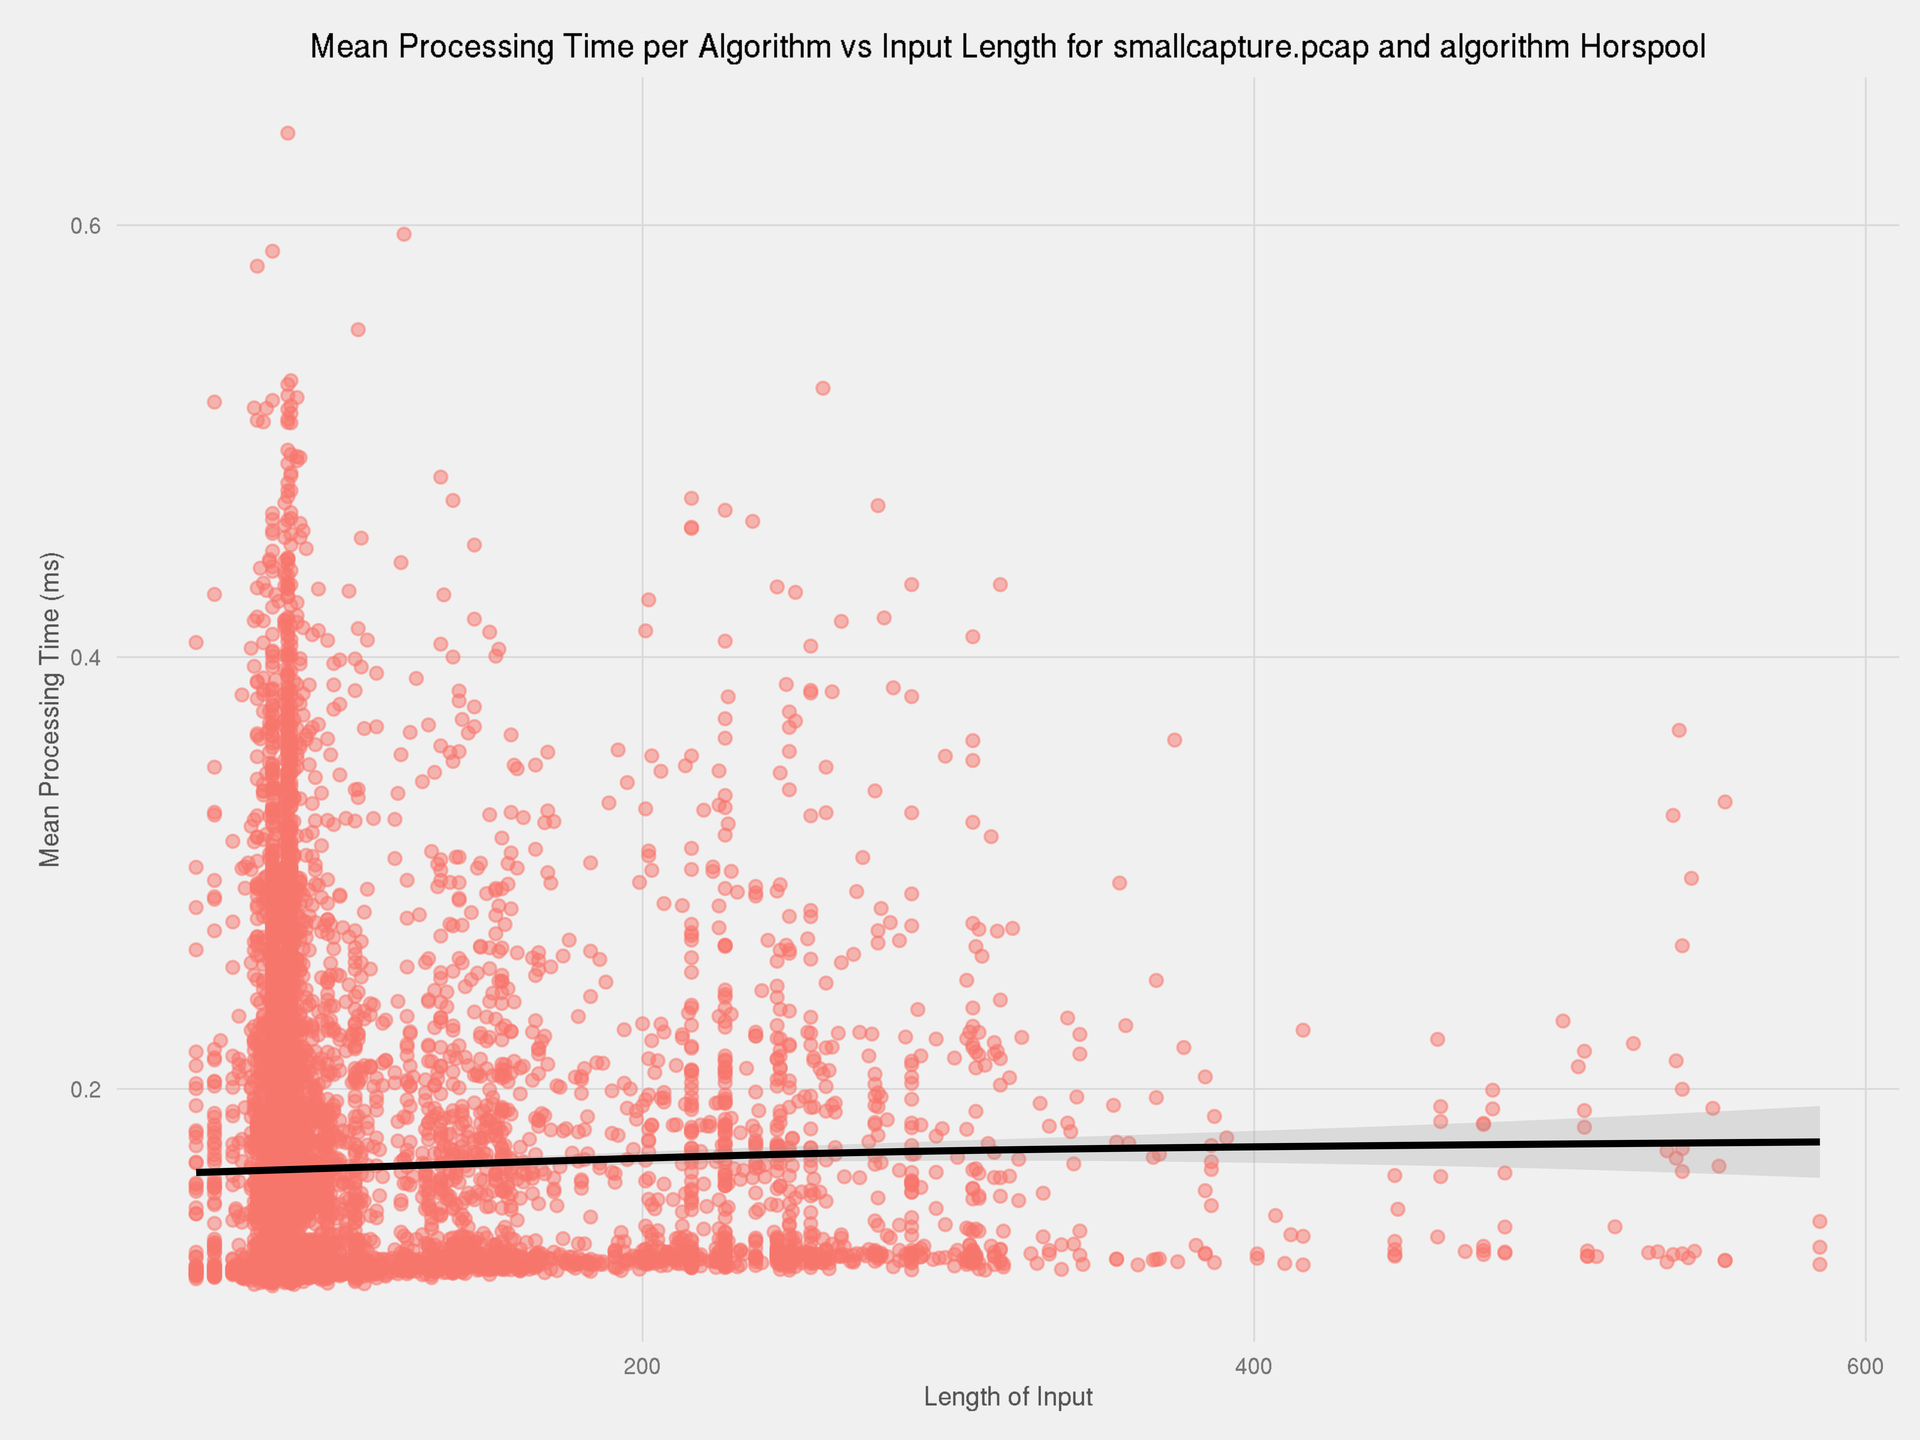
\includegraphics[width=\columnwidth]{images/scatter_mean_vs_input_length_Horspool}
  \caption{Horspool}
\end{figure}

\begin{figure}[!hbt]
  \centering
  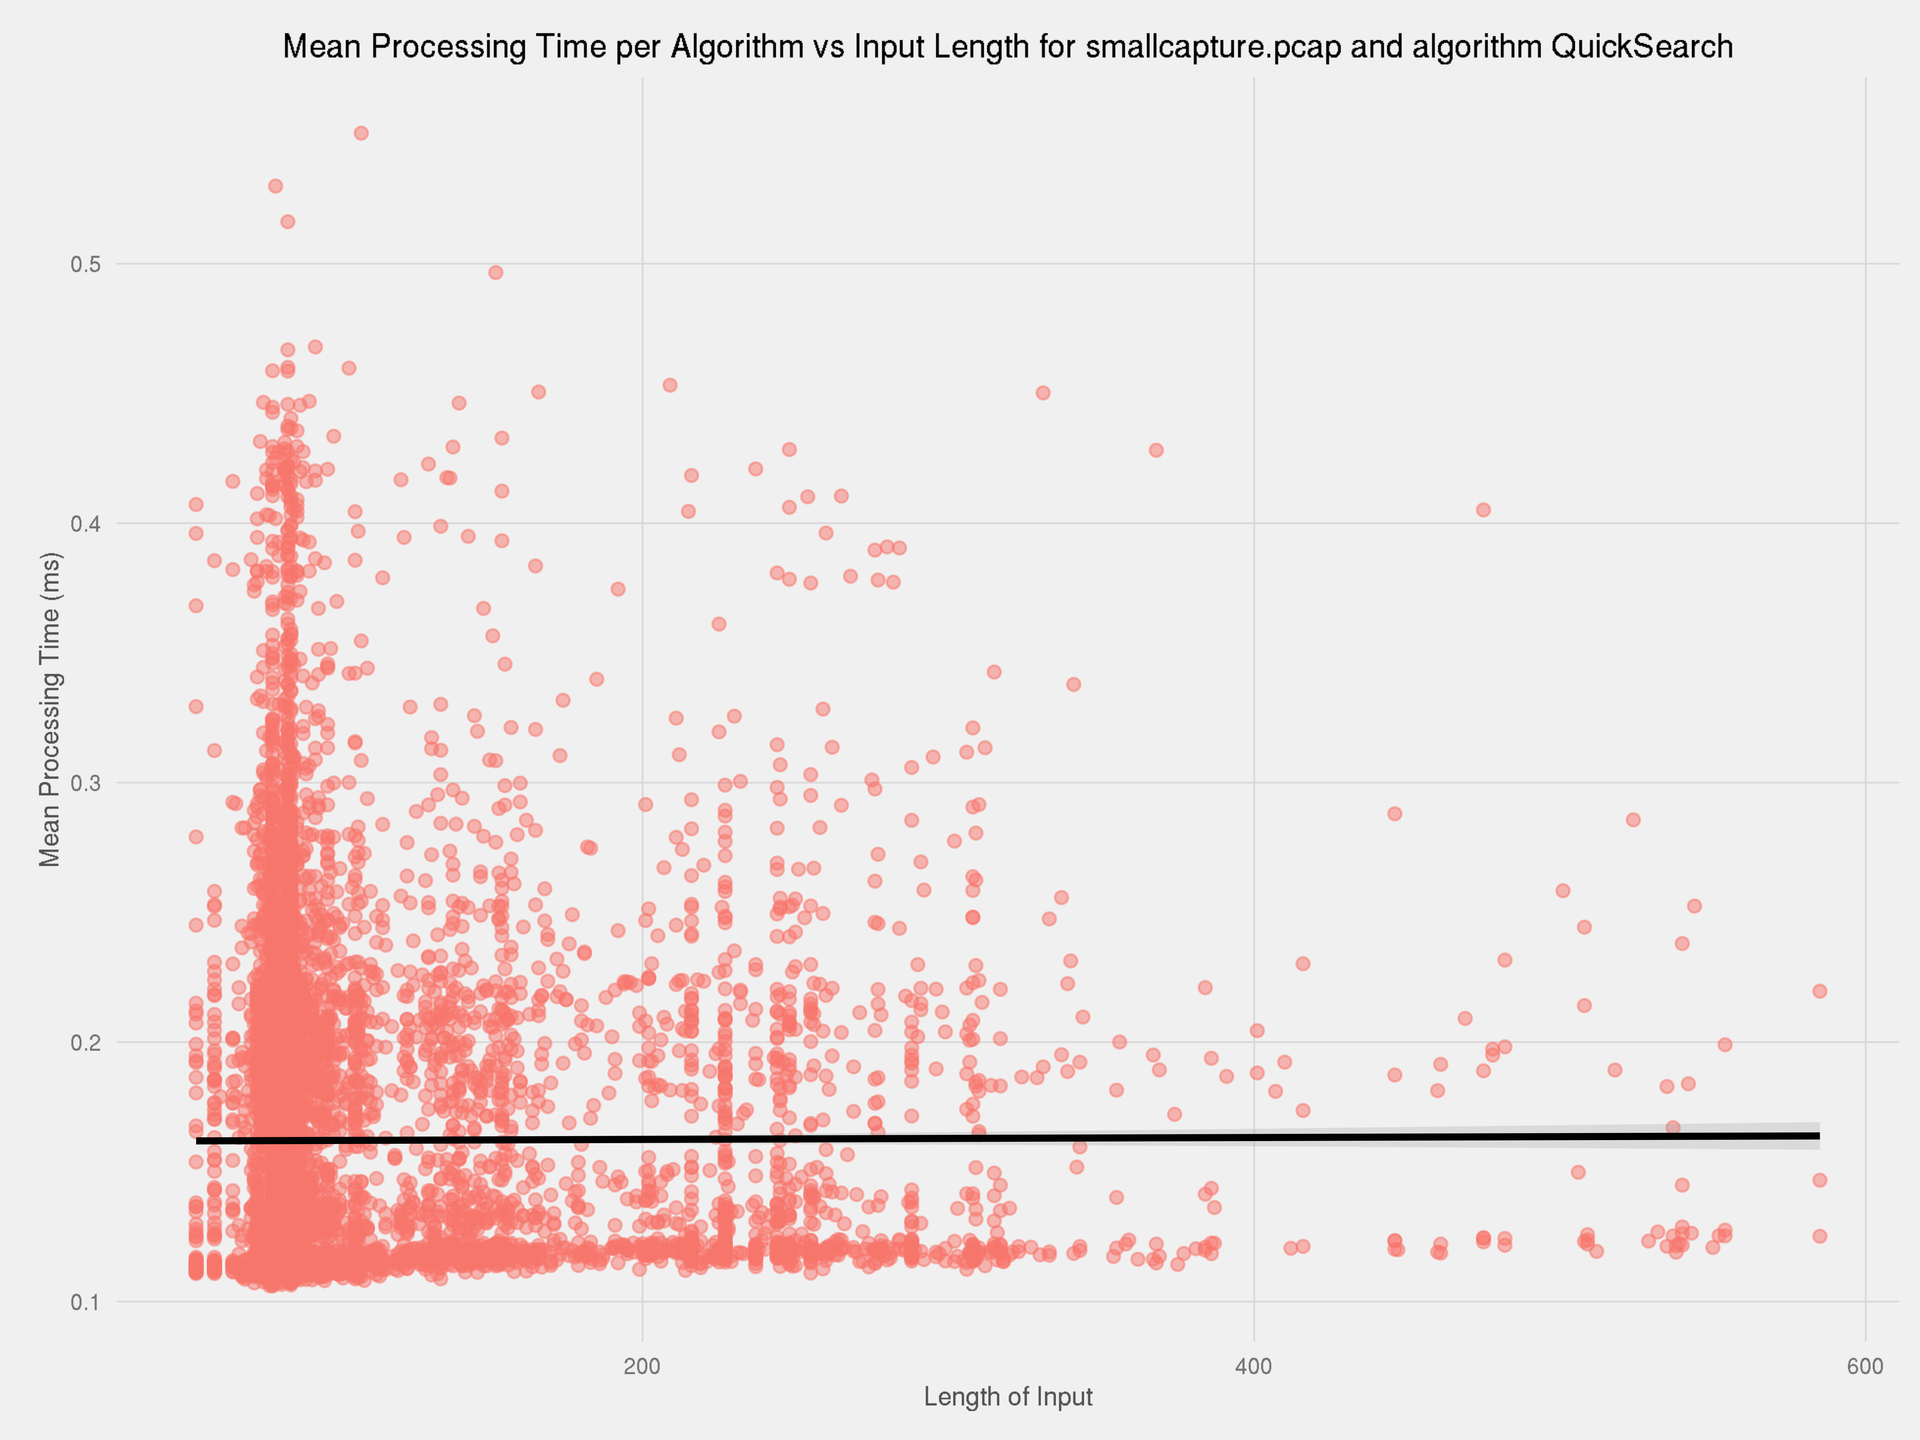
\includegraphics[width=\columnwidth]{images/scatter_mean_vs_input_length_QuickSearch}
  \caption{Quick Search}
\end{figure}

\begin{figure}[!hbt]
  \centering
  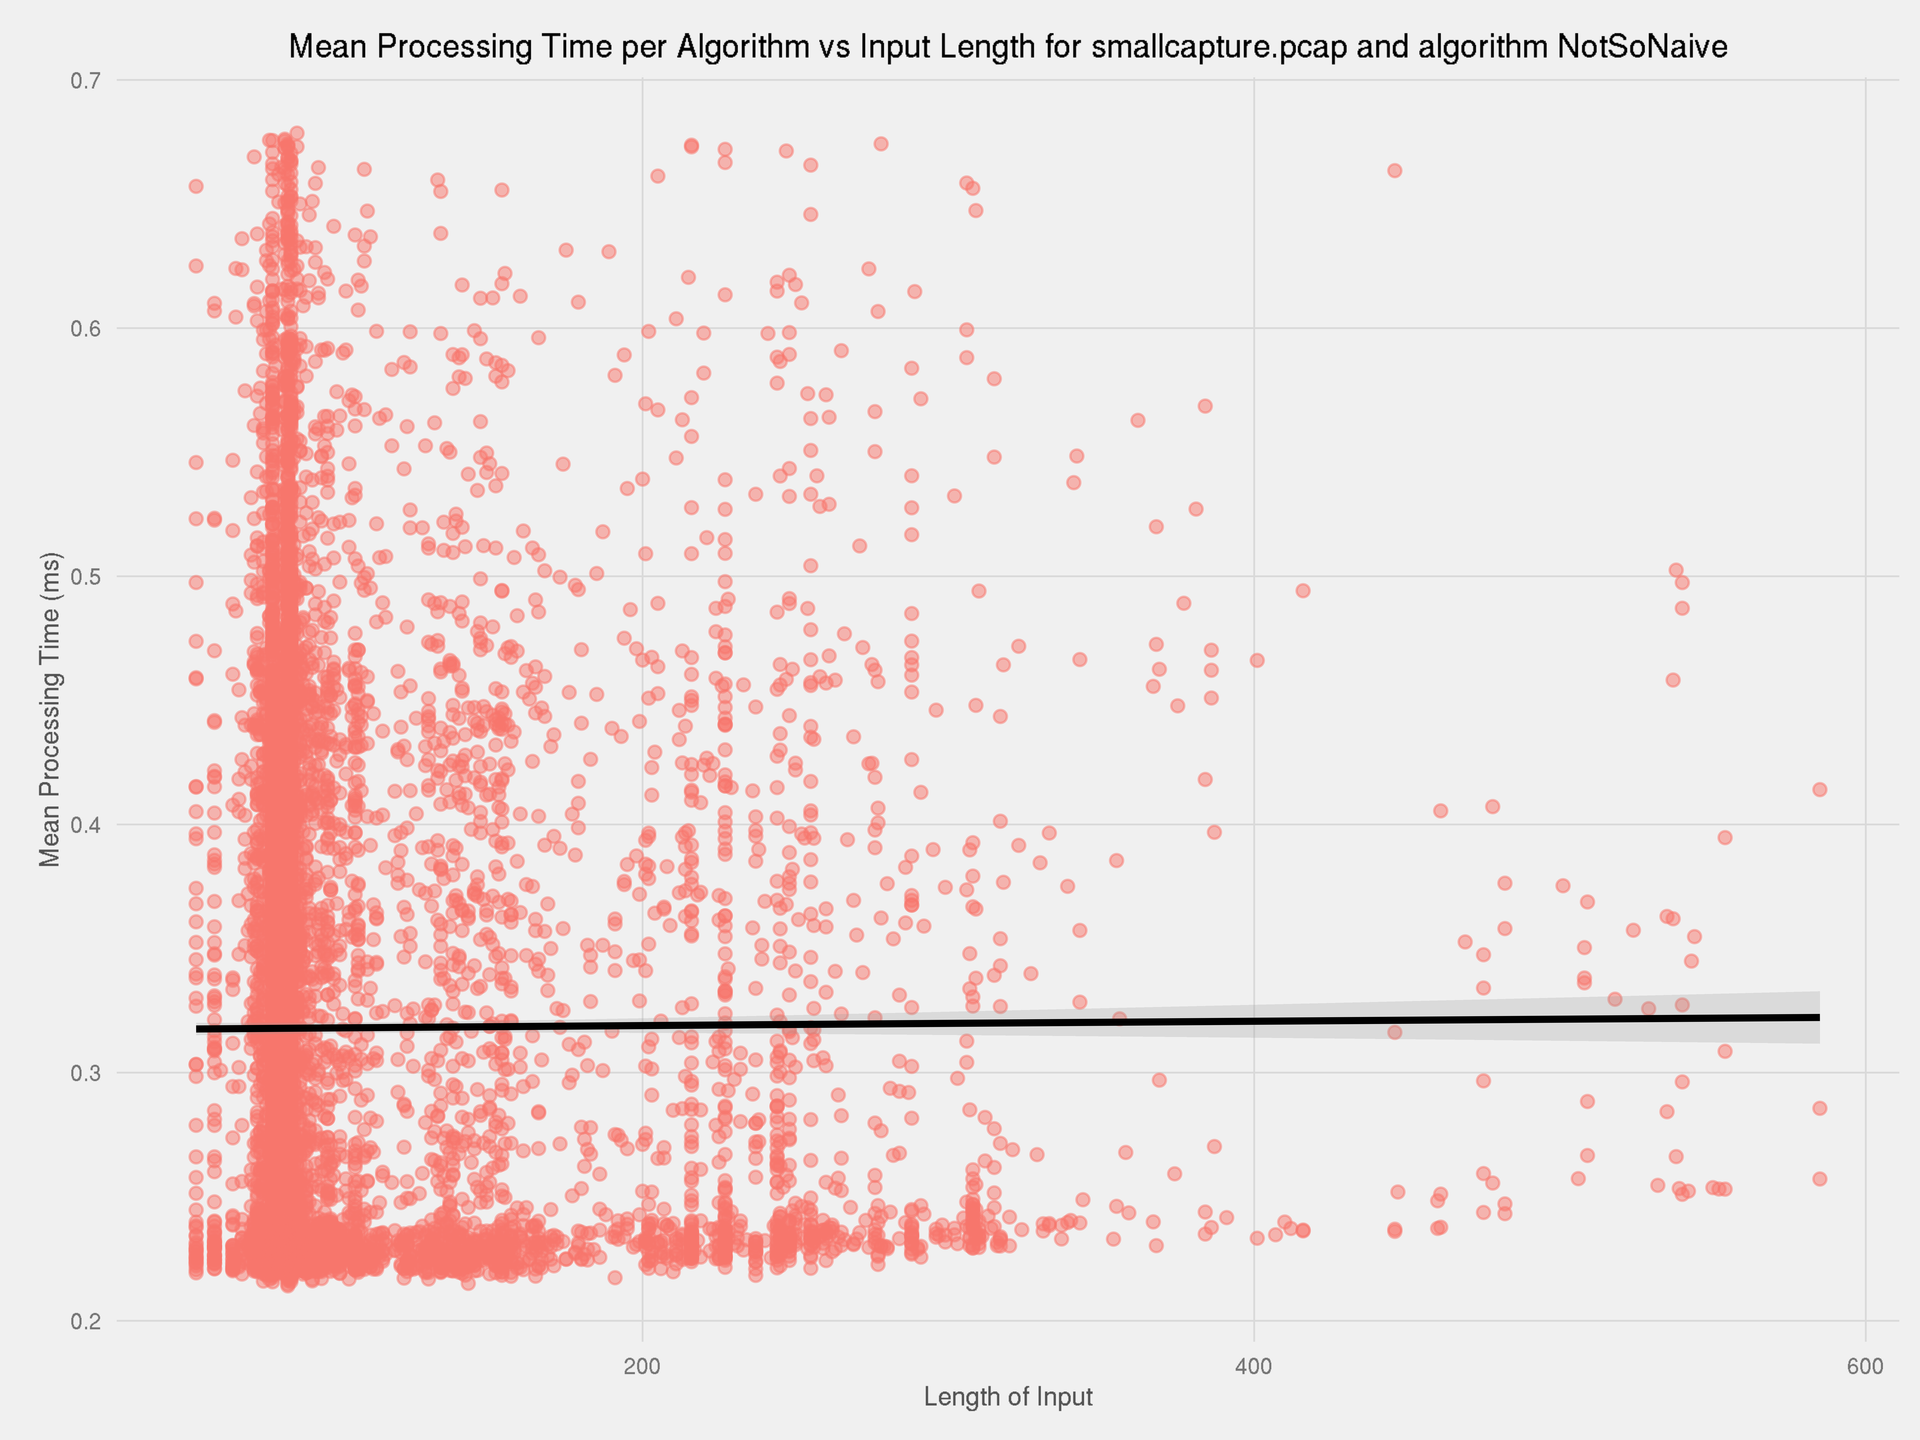
\includegraphics[width=\columnwidth]{images/scatter_mean_vs_input_length_NotSoNaive}
  \caption{Not So Na\"ive}
\end{figure}

\begin{figure}[!hbt]
  \centering
  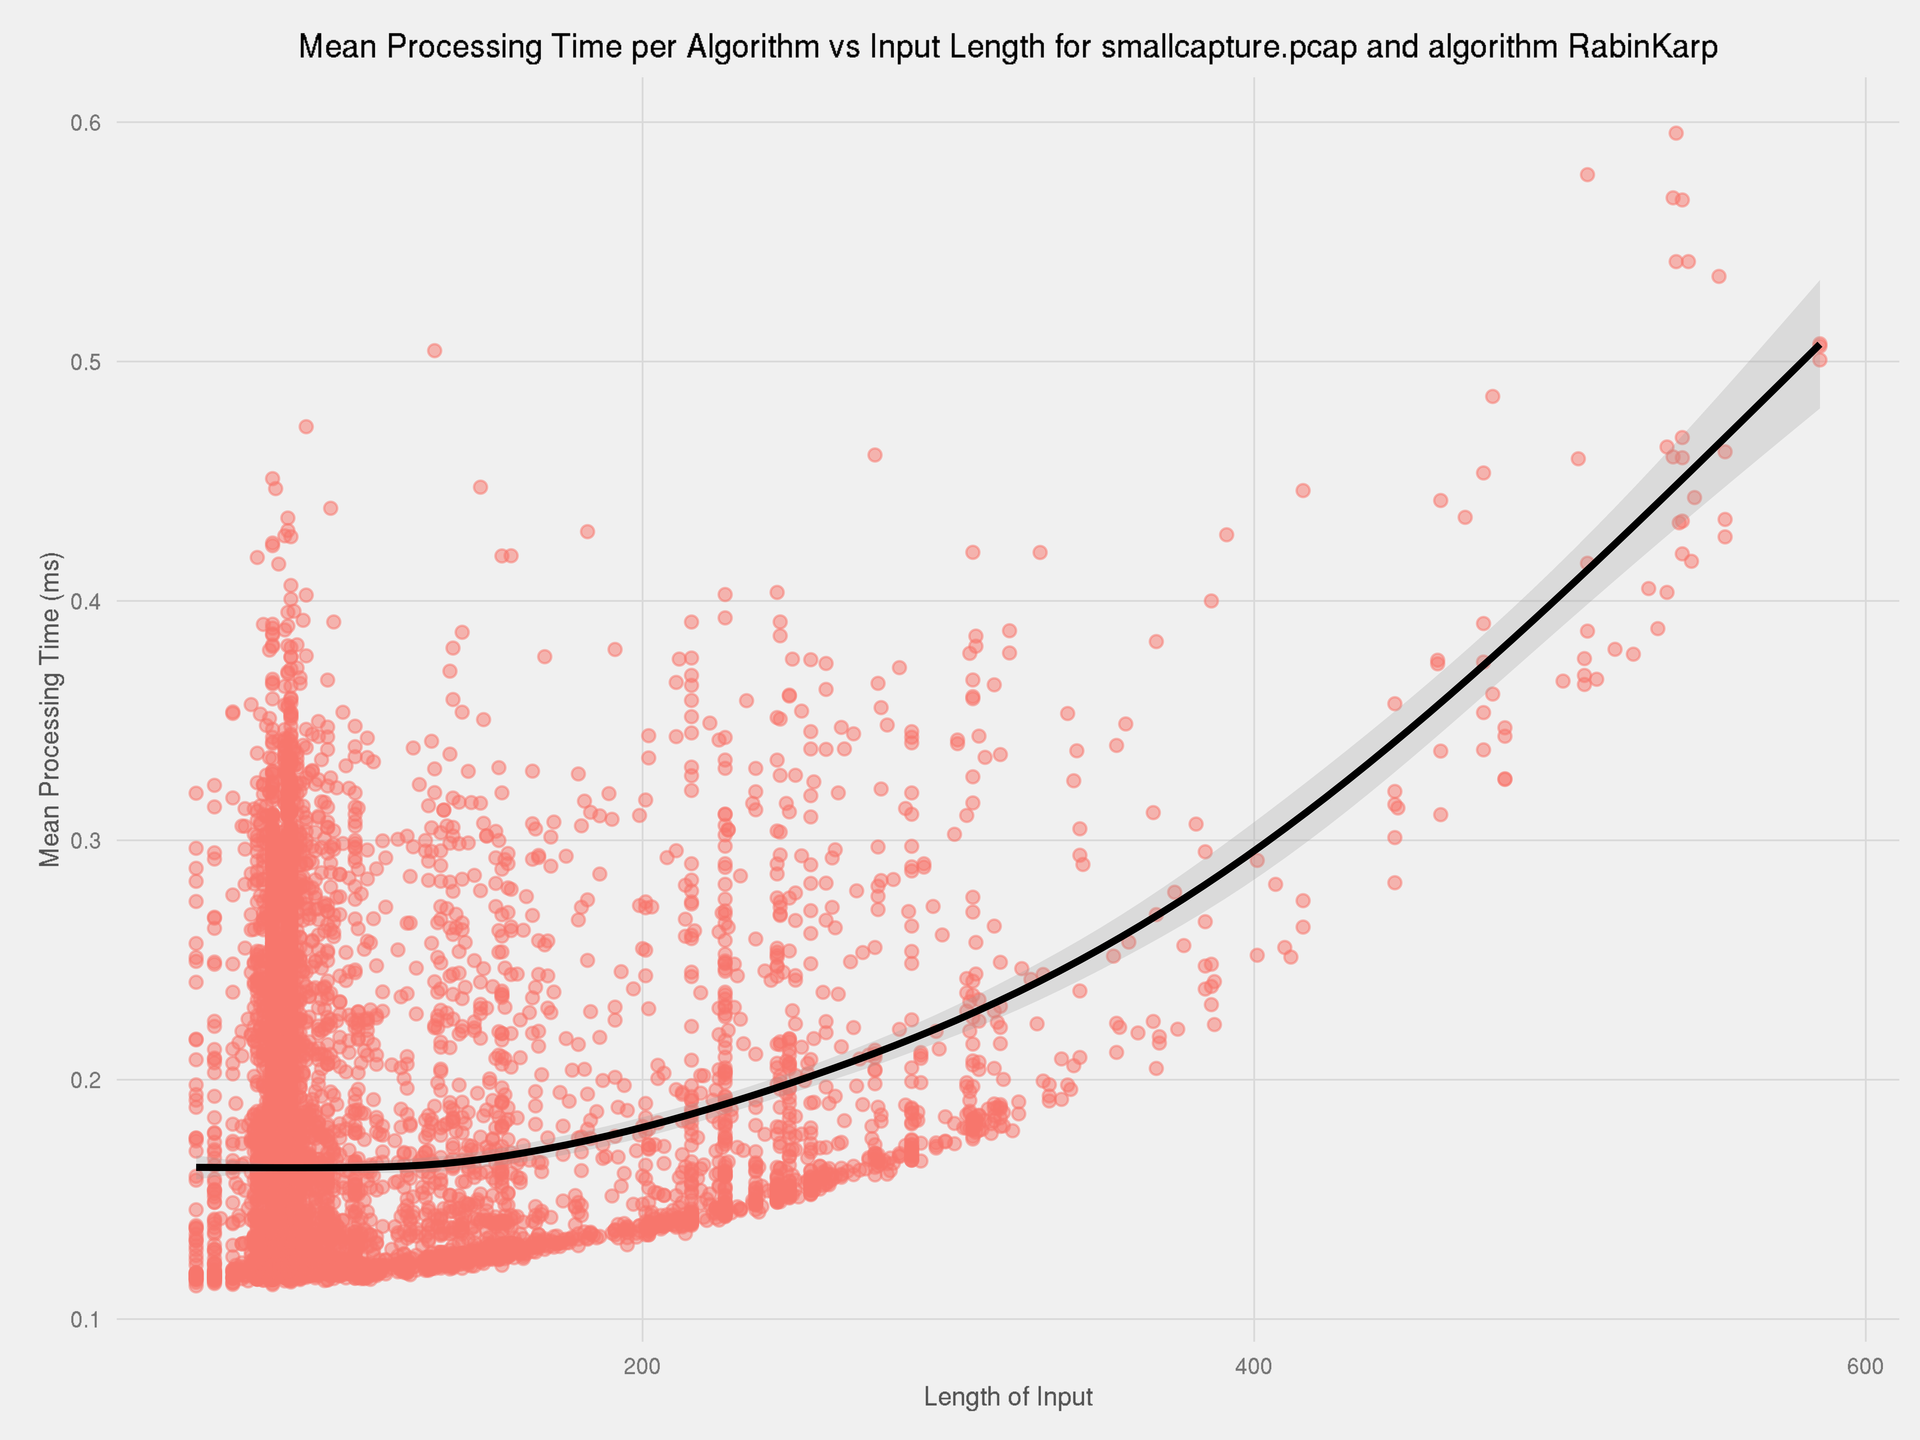
\includegraphics[width=\columnwidth]{images/scatter_mean_vs_input_length_RabinKarp}
  \caption{Rabin-Karp}
\end{figure}

Algorithms best suited to deep packet inspection would be expected to perform better for smaller input lengths and the performance at input lengths larger than the maximum length of a packet would not matter. Algorithms with a bounded maximum processing time would be especially enticing to a deep packet inspection system implementor as it could guarantee a minimum throughput. 

Figure \ref{figure-individualalgorithmsvslength} shows similar graphs to Figure \ref{figure-speedvslength} but this time just the two fastest and two slowest algorithms were chosen.

\subsubsection{Which Algorithms Have the Least Fluctuating Processing Times?}

It is important that algorithms have consistent performance. Algorithms that have highly fluctuating processing speeds lead to unpredictable processing times and unwanted slowdowns of realtime packet inspection.

Figure \ref{figure-standarddeviation} shows the standard deviations of the mean processing time for each packet each of the algorithms for \textit{Dataset A}. Most algorithms appear to have relatively low fluctuation on their processing times whilst some are a bit higher. The Horspool \citep{horspool1980} algorithm appears to have a very low standard deviation which, combined with its speed shown in Table \ref{table-algorithmspeed}, makes it a very strong packet processing algorithm compared to the other algorithms.

Interestingly in Figure \ref{figure-standarddeviation}, QuickSeach has a notably higher standard deviation than Horspool. It may not be all that well suited to packet inspection as a result.

\begin{figure}[hbt]
  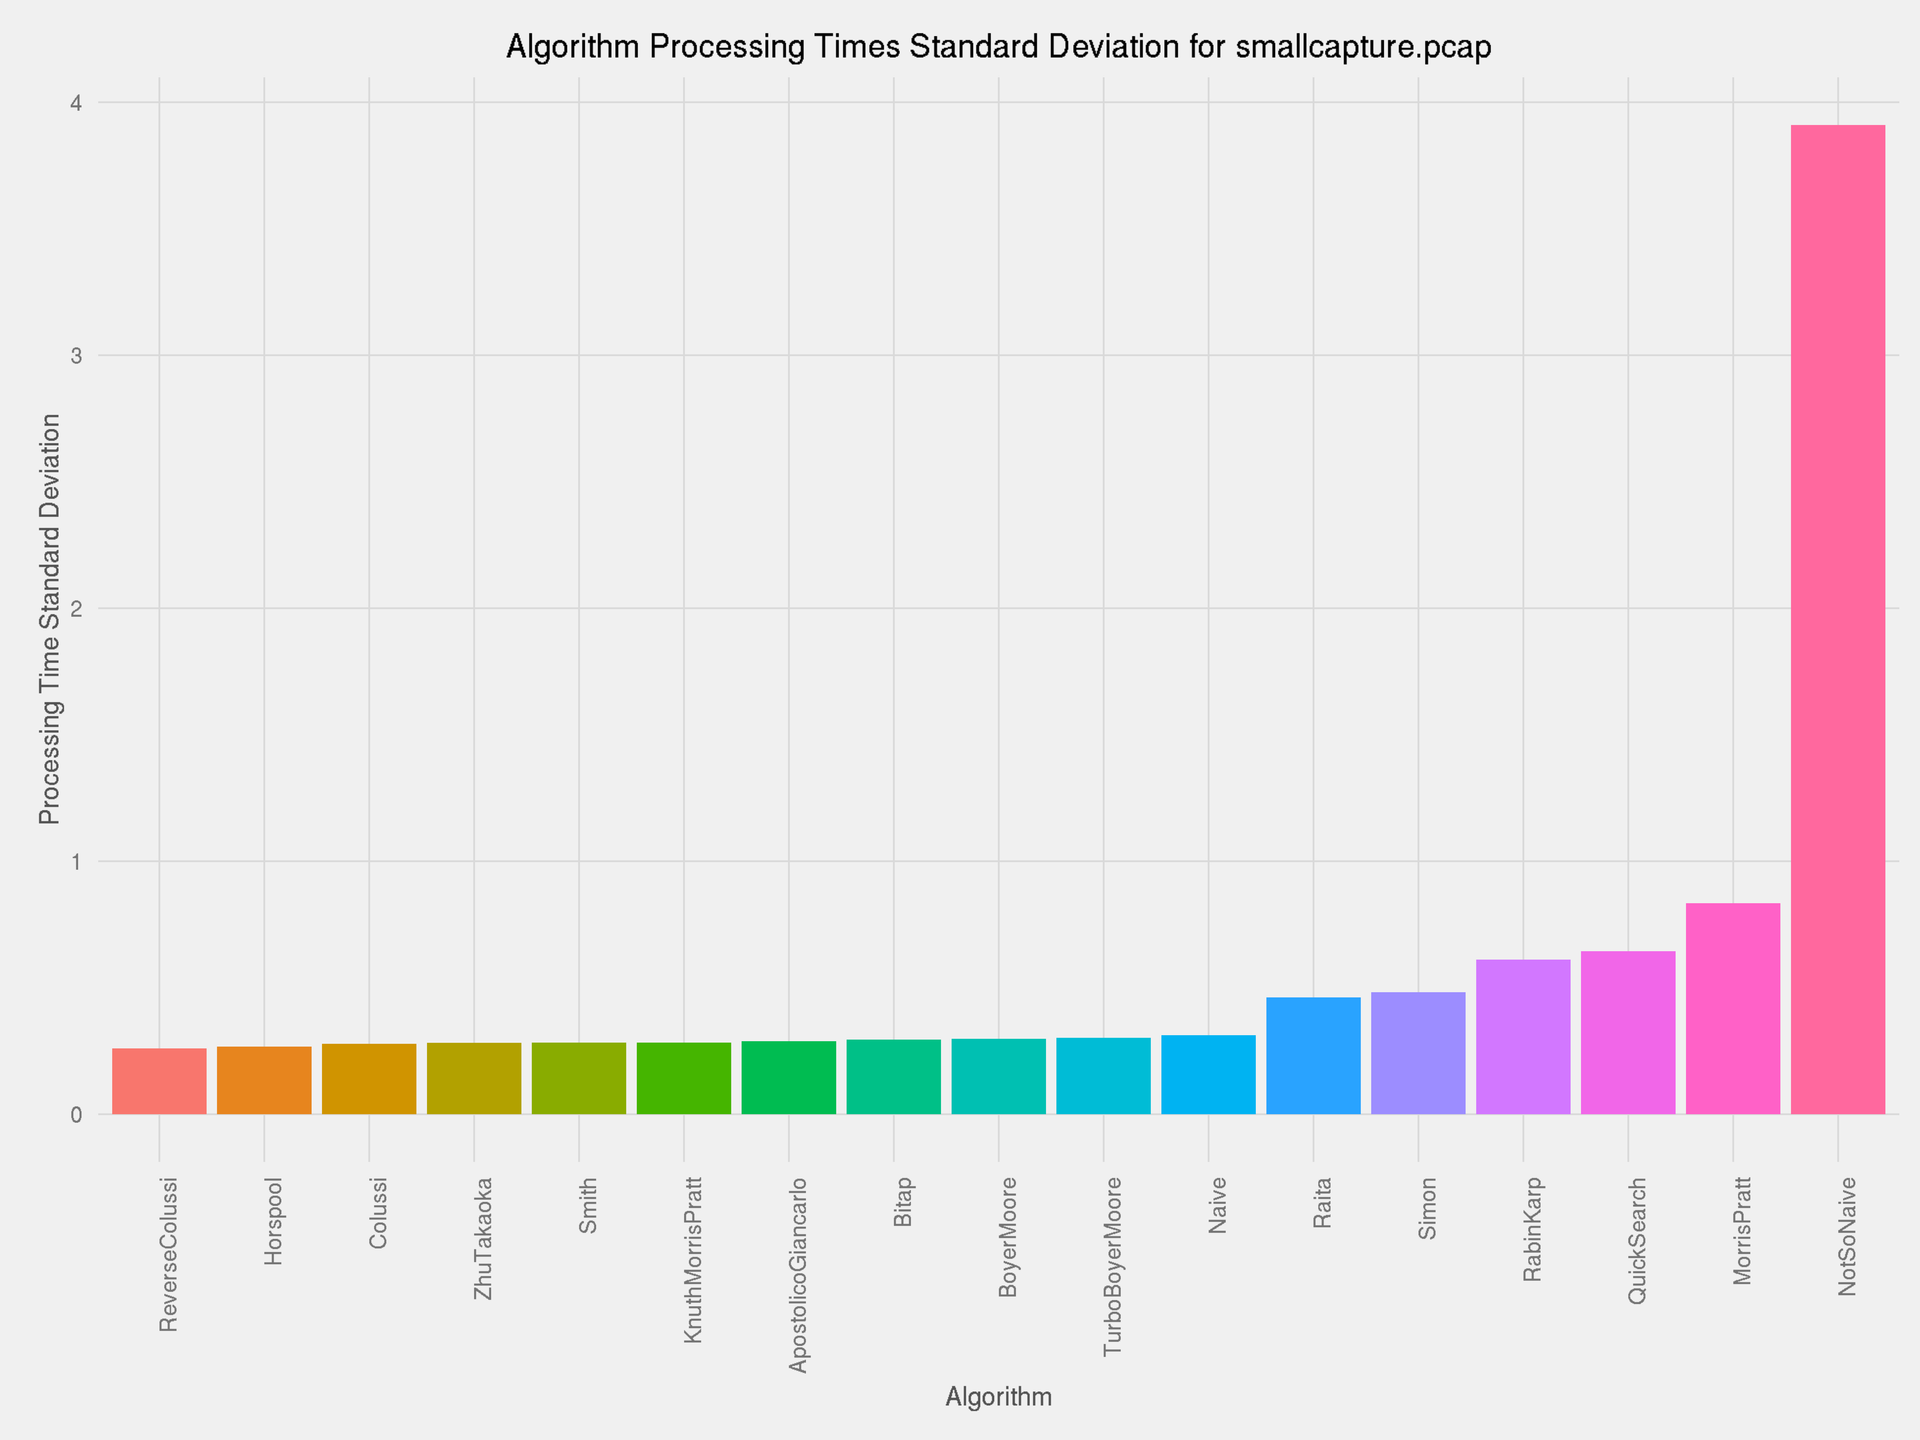
\includegraphics[width=\columnwidth]{images/bar_graph_algorithm_standard_deviation_pcap}
  \caption{The standard deviation of processing time per algorithm for \textit{Dataset A}.}
  \label{figure-standarddeviation}
\end{figure}


\subsubsection{Real World Packet Processing Speeds}

For the packet data, most algorithms have a mean packet processing speed of anywhere between 0.1 and 0.2 milliseconds.

The average processing speed of about 0.15ms (Table \ref{table-algorithmspeed}) as well as an average packet length of about 110 bytes (Table \ref{table-inputsummary}) means that a rough line speed of around 6 megabits per second is achievable. This speed is obviously much less than what would be required of a modern Deep Packet Inspection system - it is a few orders of magnitude smaller than what would be required. This research is not that concerned with the absolute speeds of each of these algorithms but their speeds when compared with each other. 

\section{Conclusion}

Of the original algorithms chosen to test, Horspool \citep{horspool1980} seems to perform best when it comes to packet analysis.
Although software-based deep packet inspection is not as popular as its hardware counterpart, it does provide an easier-to-scale environment that can better cope with the fluctuations of periodic network load. Bootstrapping a software-based packet inspection system could be done with any consumer-grade computer equipment without the need to purchase expensive hardware.

\section{Future Work}

The two datasets used in these tests are good examples of datasets from their domains. \textit{Dataset A}, which contains DNS data, represents real-world DNS traffic. The drawback of \textit{Dataset A} is that, although of normal length of DNS data, the average length of each packet is very short. The average length of each packet in \textit{Dataset A} is about 110 bytes. The maximum length of an ethernet frame is 1500 bytes \citep{law2012}. This discrepancy could serve to conceal the true nature of the algorithms.

Further work on this subject could include tests using datasets more akin the the entire spectrum of traffic seen on networks today. 

\bibliographystyle{IEEEtranS}
\bibliography{references}

\end{document}
